\section{Polarimetría}
\subsection{Polarización}
\begin{frame}{\secname : \subsecname}
  \begin{figure}
    \centering
    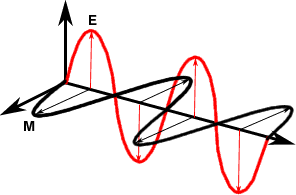
\includegraphics[scale=0.7]{fig:onda}
    \caption{Algunos SAR pueden emitir y recibir tanto en H como en V. Combinado distintas emisiones y recepciones se obtienen 4 combinaciones polarimétrica:{\bf HH HV VH y VV}}
    \label{}
  \end{figure}
\end{frame}
%--- Next Frame ---%

\begin{frame}{\secname : \subsecname}
  \begin{figure}
    \centering
    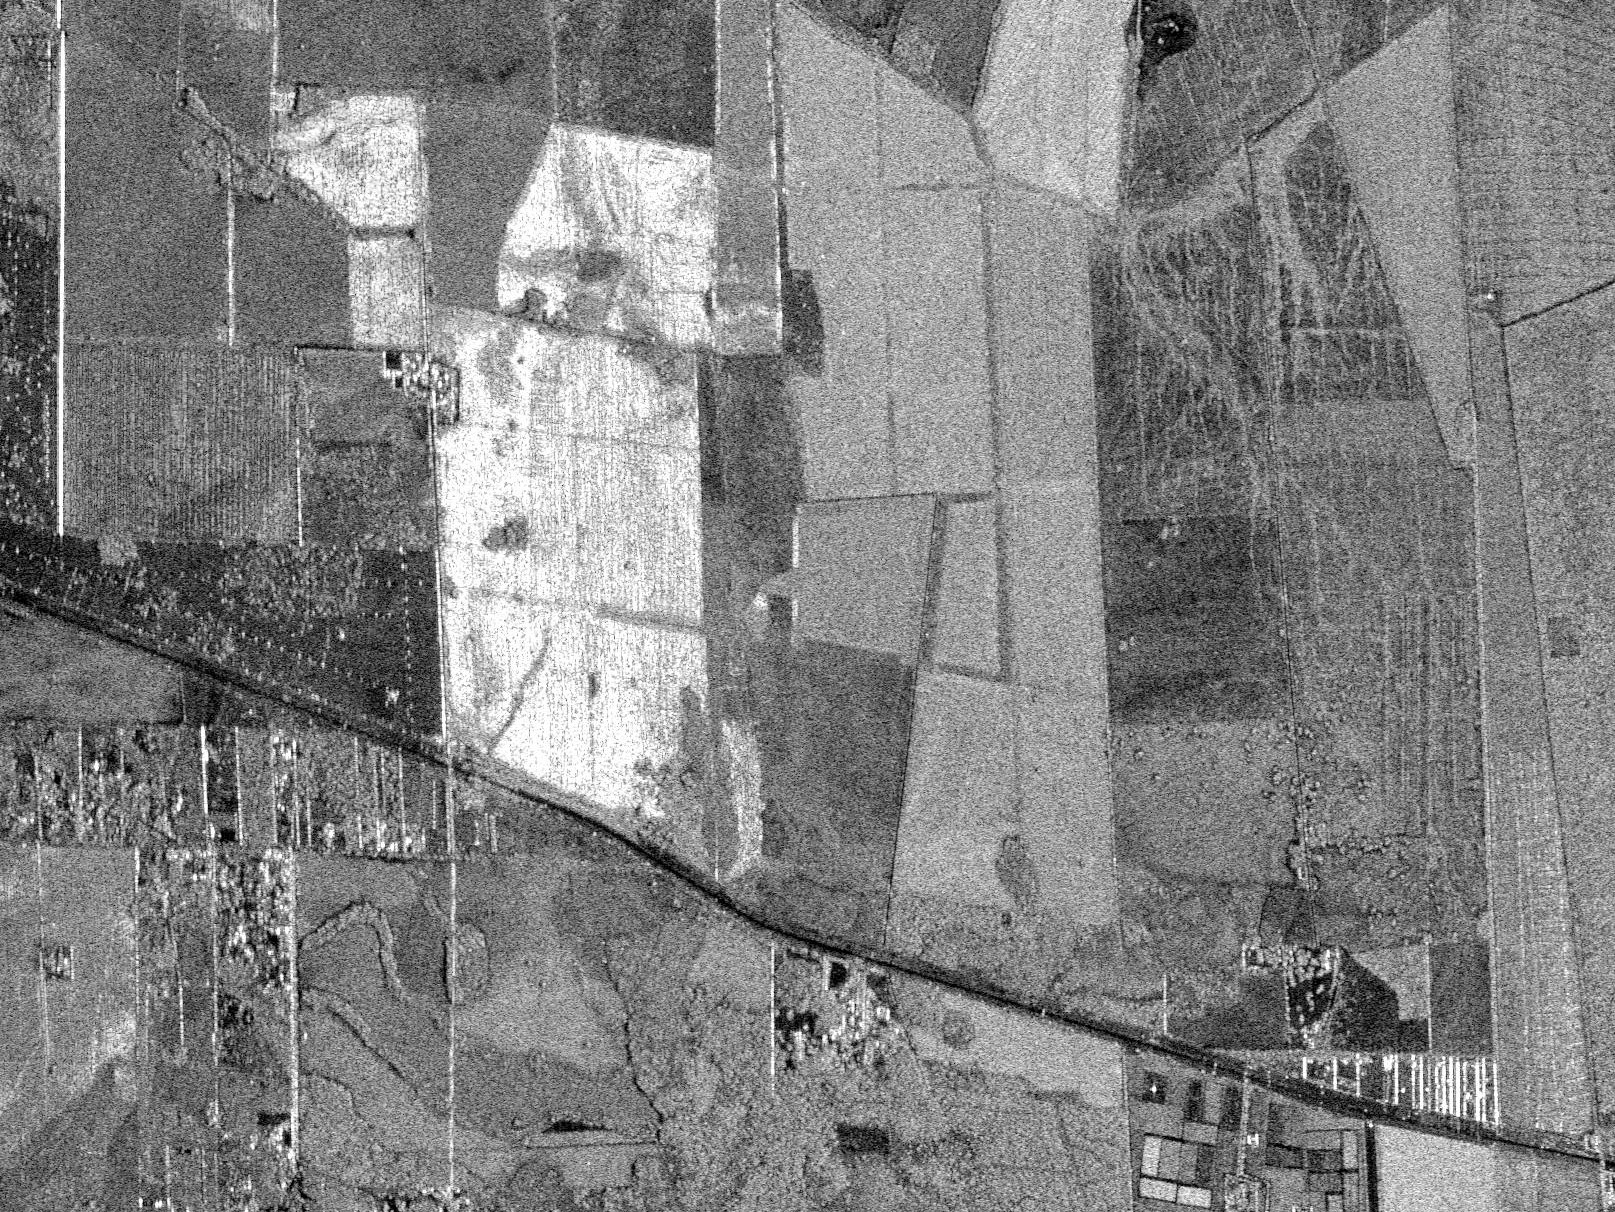
\includegraphics[scale=0.7]{fig:HH}
    \caption{HH}
    \label{}
  \end{figure}
\end{frame}
%--- Next Frame ---%

\begin{frame}{\secname : \subsecname}
  \begin{figure}
    \centering
    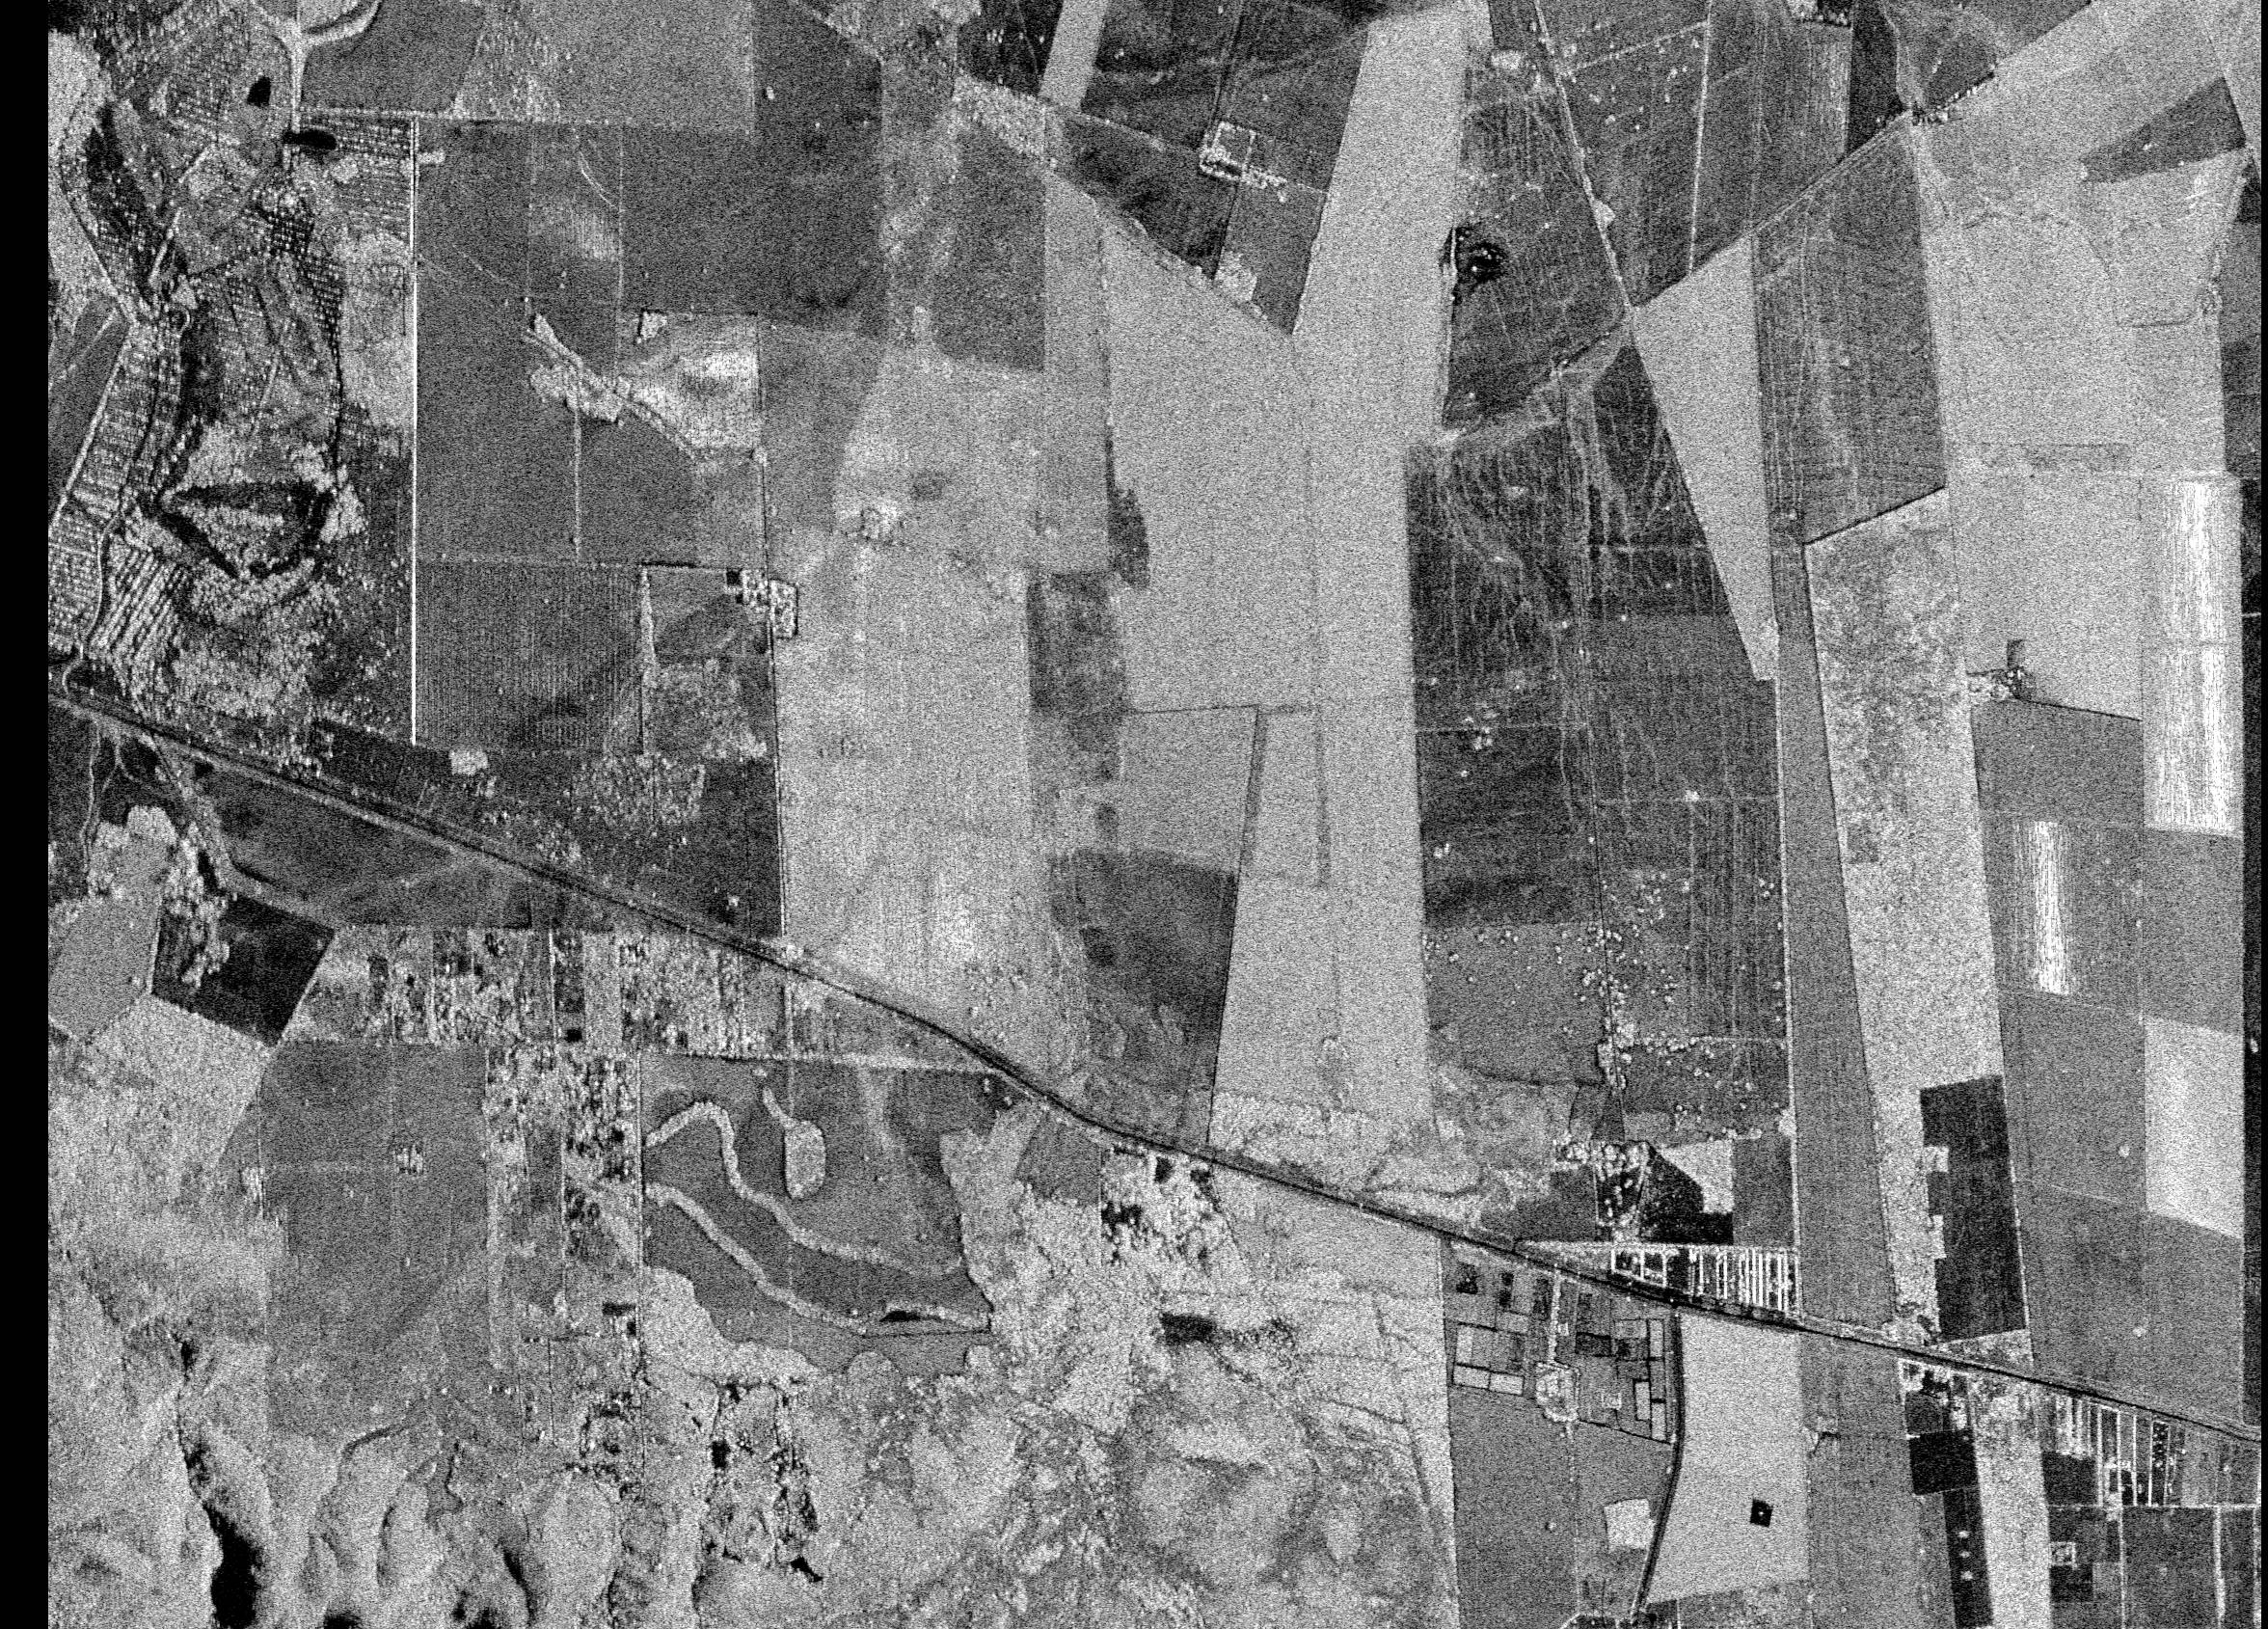
\includegraphics[scale=0.7]{fig:HV}
    \caption{HV}
    \label{}
  \end{figure}
\end{frame}
%--- Next Frame ---%

\begin{frame}{\secname : \subsecname}
  \begin{figure}
    \centering
    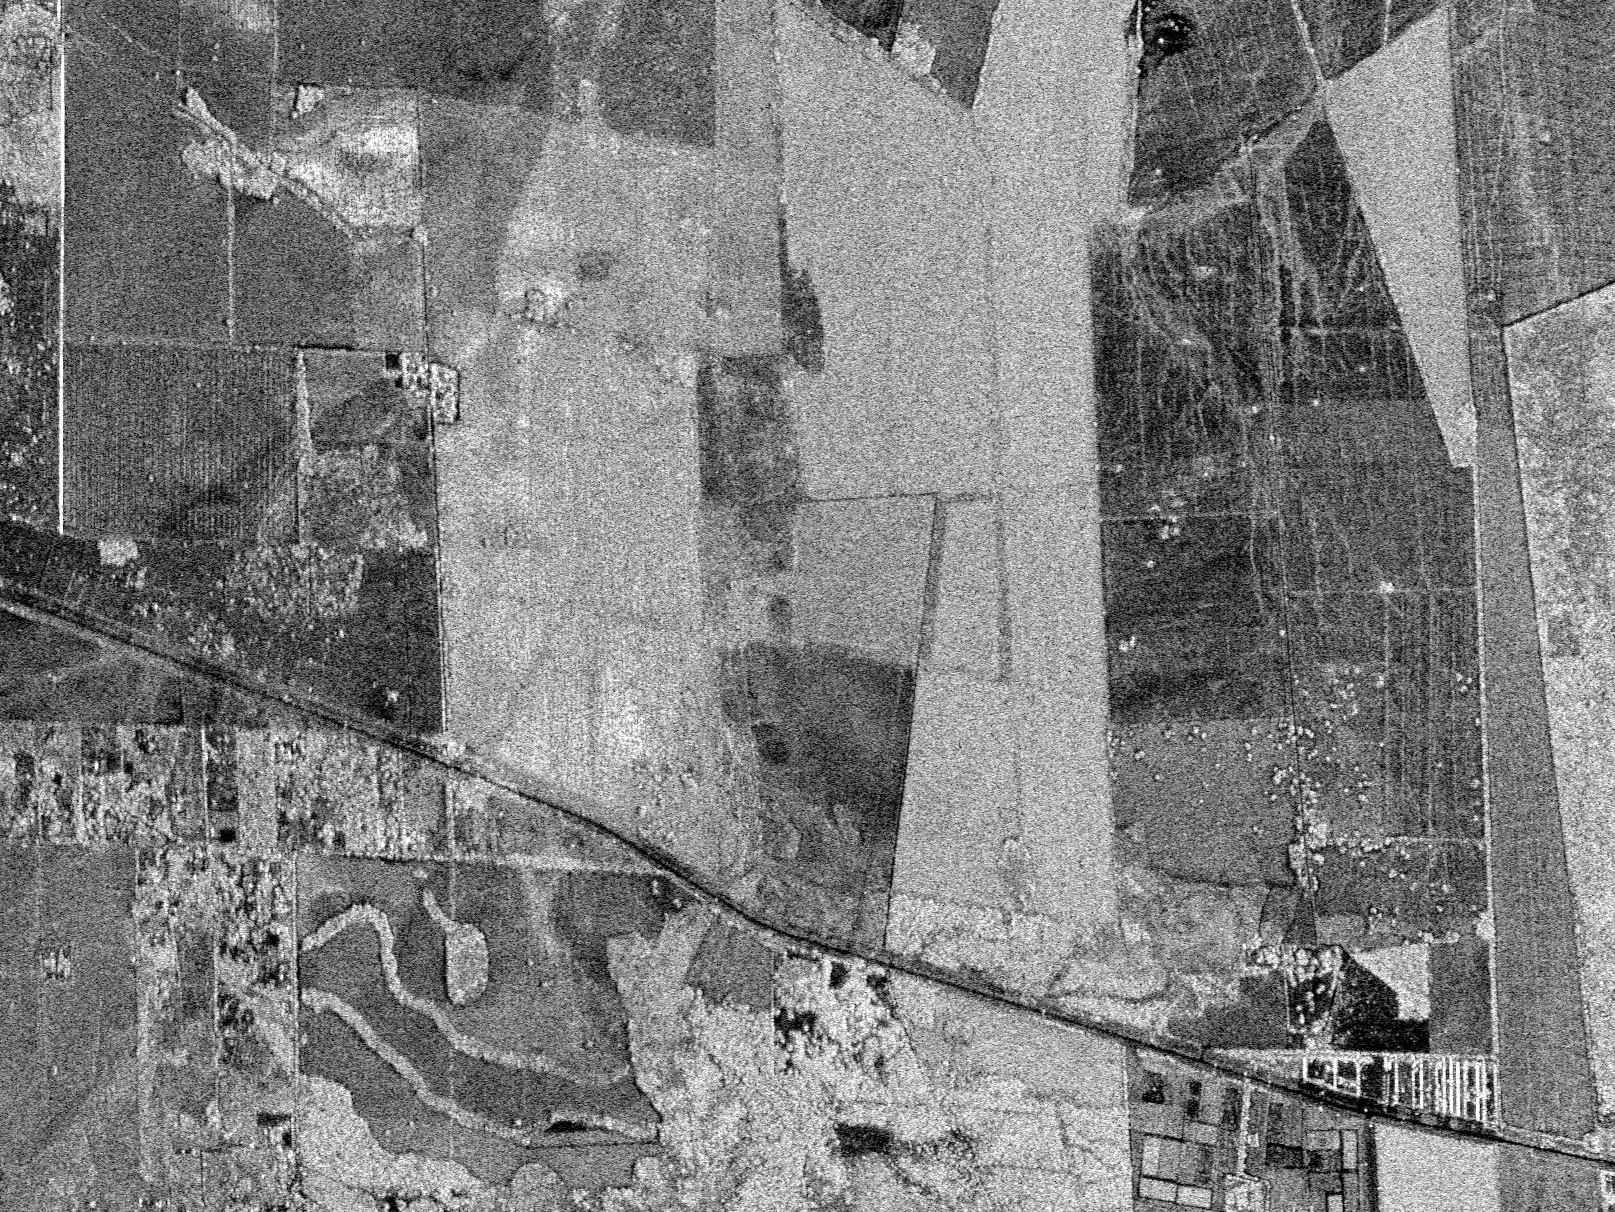
\includegraphics[scale=0.7]{fig:VH}
    \caption{VH}
    \label{}
  \end{figure}
\end{frame}
%--- Next Frame ---%

\begin{frame}{\secname : \subsecname}
  \begin{figure}
    \centering
    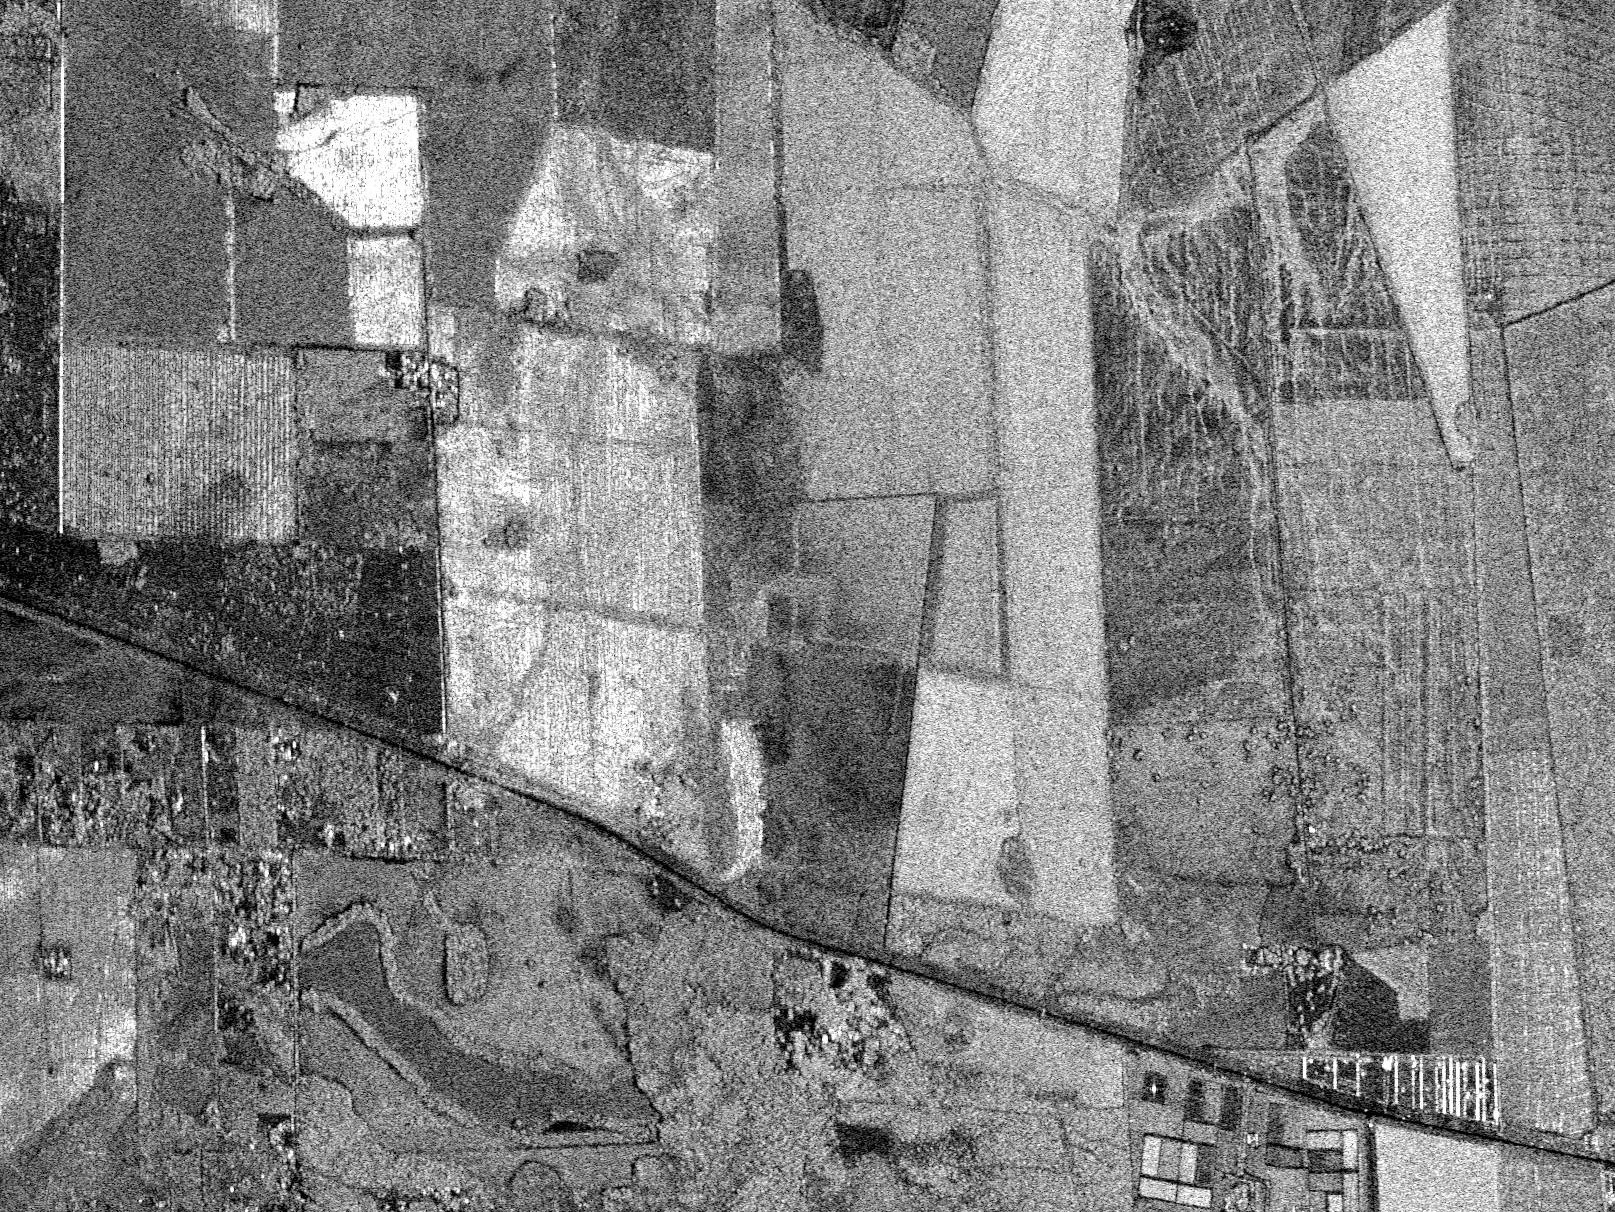
\includegraphics[scale=0.7]{fig:VV}
    \caption{VV}
    \label{}
  \end{figure}
\end{frame}
%--- Next Frame ---%

\begin{frame}{\secname : \subsecname}
  \begin{columns}
    \begin{column}{0.5\textwidth}
     \begin{block}{??}
      \begin{equation}
        S=
  \begin{bmatrix}
    S_{HH} & S{HV} \\
    S_{VH} & S{VV}
  \end{bmatrix}
      \end{equation}
     \end{block}
    \end{column}
    \begin{column}{0.5\textwidth}  %%<--- here
      \begin{block}{Matriz de backscatter}
        \begin{equation}
          \sigma_0=
  \begin{bmatrix}
    |S_{HH}|^2 & |S{HV}|^2 \\
    |S_{VH}|^2 & |S{VV}|^2
  \end{bmatrix}
        \end{equation}
      \end{block}
    \end{column}
    \end{columns}
\end{frame}
%--- Next Frame ---%

\begin{frame}{\secname : \subsecname}
  \begin{figure}
    \centering
    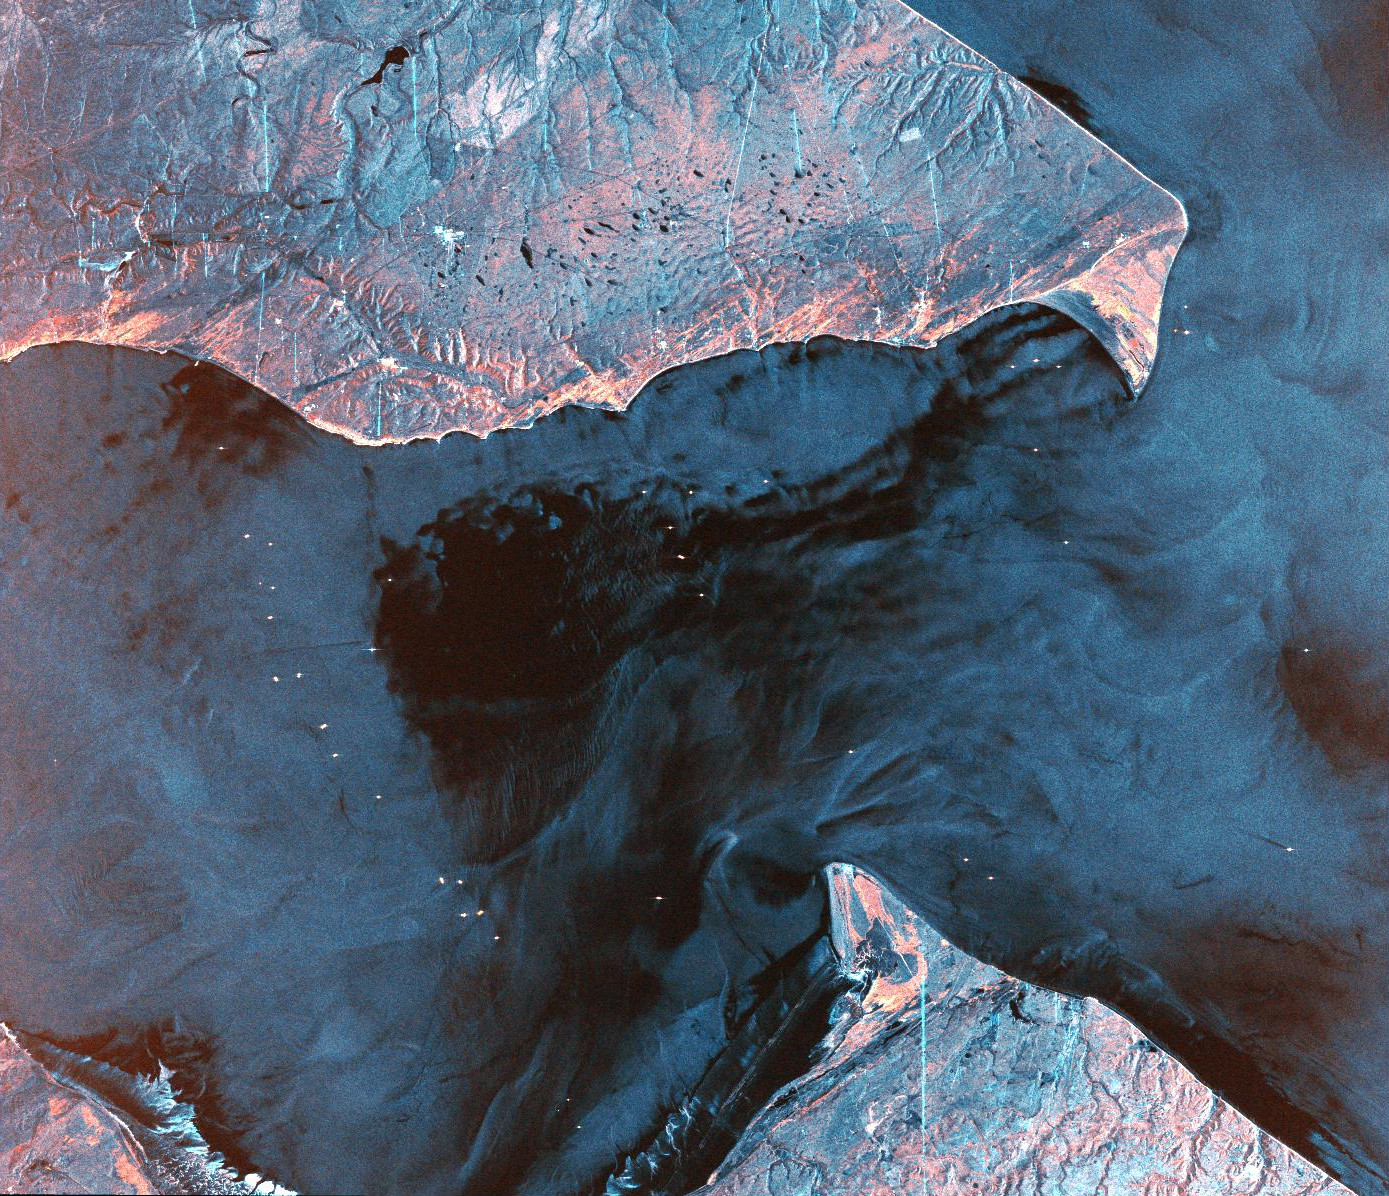
\includegraphics[scale=0.7]{fig:rgbpol}
    \caption{Rojo: HV, Verde: HH, Azul: HH-VV}
    \label{}
  \end{figure}
\end{frame}
%--- Next Frame ---%

\subsection{Descoposición de Pauli}

\begin{frame}{\secname : \subsecname}
  \begin{columns}
    \begin{column}{0.5\textwidth}
     \begin{block}{??}
      \begin{equation}
        R = \left(\frac{HH-VV}{\sqrt{2}}\right)^2
      \end{equation}
      \begin{equation}
        G = \left(\sqrt{2}HV\right)^2
      \end{equation}
      \begin{equation}
        R = \left(\frac{HH+VV}{\sqrt{2}}\right)^2
      \end{equation}
     \end{block}
    \end{column}
    \begin{column}{0.5\textwidth}  %%<--- here
      \begin{figure}
        \centering
        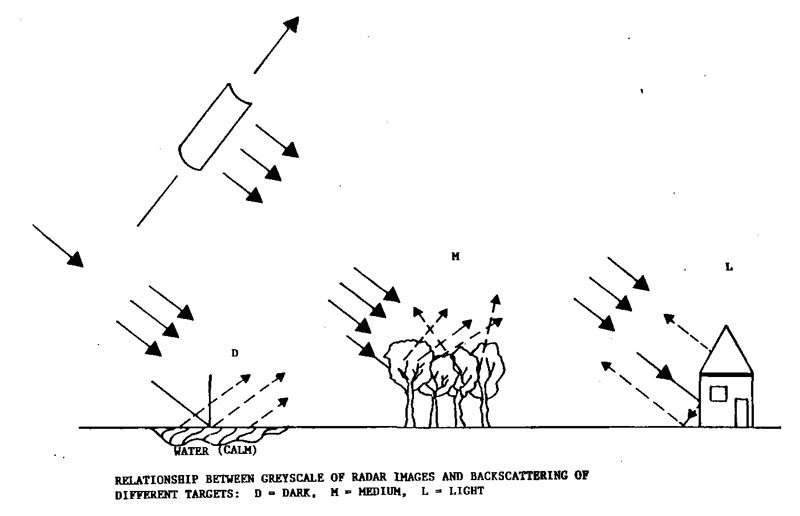
\includegraphics[height=0.7\textheight]{fig:pauli.png}
        \caption{}
        \label{}
      \end{figure}
    \end{column}
    \end{columns}
    La descomposición de Pauli es una manera de visual de ver los distintos mecanismo de scattering presentes
\end{frame}
%--- Next Frame ---%

\begin{frame}{\secname : \subsecname}
  \begin{figure}
    \centering
    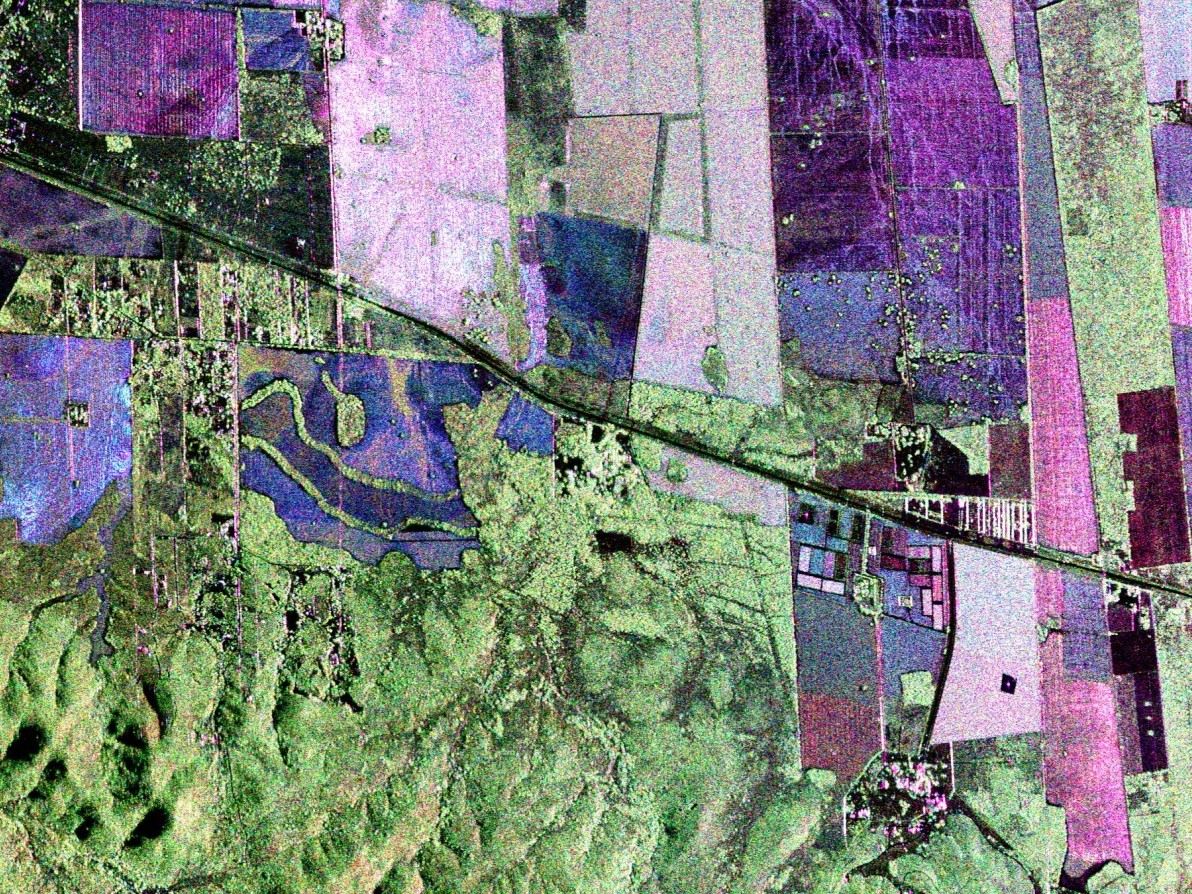
\includegraphics[scale=0.7]{fig:rgbpauli}
    \caption{}
    \label{}
  \end{figure}
\end{frame}
%--- Next Frame ---%
